\begin{frame}
  \frametitle{Developing a Computational Methodology}
  \begin{figure}[h!]
    \centering
    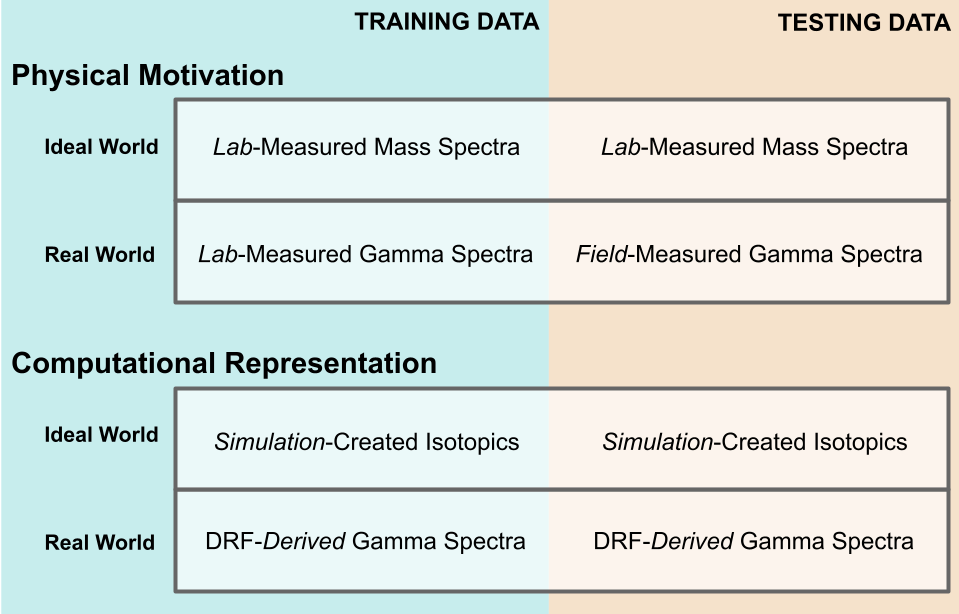
\includegraphics[width=0.9\textwidth]{./figures/project_design.png}
    \caption{Illustration of the computational project design rationale}
  \end{figure}
\end{frame}

\begin{frame}
  \frametitle{Experimental Design Overview}
  \begin{minipage}{0.45\textwidth}
    \begin{figure}
      \centering
      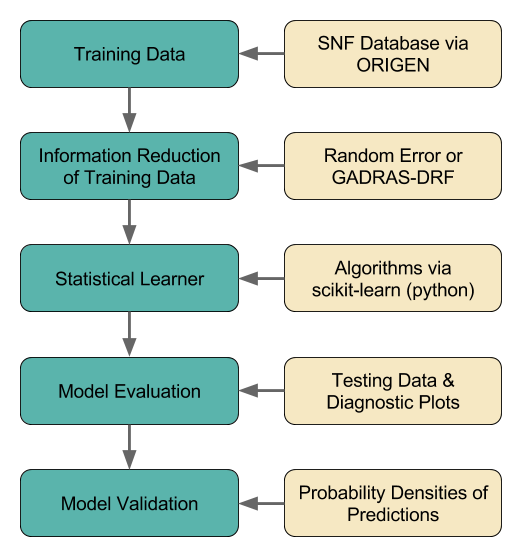
\includegraphics[height=0.5\textheight]{./figures/methodology.png}
      \caption{Workflow of a computational methodology using statistical models}
    \end{figure}
  \end{minipage}%
  \begin{minipage}{0.55\textwidth}
    \begin{itemize}
      \item Training Data: SNF recipes from SCALE/ORIGEN-ARP \cite{scale, origen}
      \item Information Reduction
        \begin{itemize}
          \item Nuclide Masses: Random error injection
          \item Nuclide Activities: Generate computational gamma spectra from GADRAS \cite{gadras}
        \end{itemize}
      \item Statistical Methods
        \begin{itemize}
          \item Machine learning algorithms (kNN \& Decision Trees) \cite{scikit}
          \item Maximum likelihood calculation method \cite{mll_method, mll_sensitivity}
        \end{itemize}
      \item Performance
        \begin{itemize}
          \item Test cases from SFCOMPO \cite{sfcompo}
          \item Prediction error analysis
        \end{itemize}
    \end{itemize}
  \end{minipage}
\end{frame}

